\section{The mechanism}\label{sec:mech}

We follow the handle-packing scheme of \cite{OpenAI2026}. Give $\CP^2$ the Fubini--Study form for which a line has
area $1$, so that $\vol\CP^2=\frac12$ and the complement of a line is $\Bo(1)$. Let $E\subset\CP^2$ be a smooth cubic,
of area $3$. Biran \cite{Biran2001} showed that the complement of an isotropic skeleton in $\CP^2$ is symplectomorphic to
a disc bundle over $E$: the normal bundle, of degree $E\cdot E=9$, with fibre discs of capacity $\frac13$. With fibre
moment $p=\pi|w|^2$, the base area of the circle bundle at level $p$ is
\[
 A(p)=3-9p=3(1-3p)\qquad(0\le p<\tfrac13),\qquad \int_0^{1/3}A(p)\,dp=\frac12=\vol\CP^2 .
\]
The cubic is the first smooth plane curve with the topology needed by the handle construction: its base must carry a
closed one-form with nonzero period around the handle, which $H^1(S^2;\R)=0$ rules out for a line or a conic. The fibre
bound $\frac13$, and hence the condition $3c_i<C$, reflects this choice. The target capacity is $1$; the general case follows
by the dilation of Definition~\ref{def:ham-normalise}. The toric balls and the cap integral below are stated for fibres
$\C^m$, $m=n-1$; in this paper $n=2$ and $m=1$.

\subsection{Toric balls and area profiles}\label{sec:mech-toric}

On $\C^m$ let $p_j=\pi|w_j|^2$, $|p|=\sum_jp_j$ and $\omega_V=\sum_jdx_j\wedge dy_j=\sum_jdp_j\wedge d\theta_j$ (angles of period one). In dimension four the moment interval is $\Delta=[0,h]$ with $h<\frac13$, and
$V_\Delta=\{w\in\C:p(w)\le h\}=\bar D(h)$; the source caps stay in $\{p\le a_i\}$ with $a_i<h$, away from the outer
boundary $p=h$.

\begin{definition}[Toric ball]\label{def:mech-toric-ball}
\lean{OAI.PackingSufficiencySupport.closedBall,
OAI.PackingSufficiencySupport.Hamiltonian.splitCapacityBall,
OAI.PackingSufficiencySupport.Hamiltonian.complexSplitPhase_capacity}
In $\C^n=\C\times\C^m$, put $\varpi=\pi|z_{\rm b}|^2$. The ball of capacity $a$ is
$B(a)=\{\varpi+|p|\le a\}$. At a fibre point with $|p|\le a$, its base slice is a disc of capacity $a-|p|$; its slice height is $0$ for $|p|>a$. Thus the slice-height function is $(a-|p|)_+$.
\end{definition}

\begin{lemma}[The cap integral]\label{lem:mech-toric-volume}
\lean{OAI.PackingSufficiencySupport.integral_simplex_tent, OAI.PackingSufficiencySupport.integral_tent}
For $a\ge0$,
\[
 \int_{\R^m_{\ge0}}(a-|p|)_+\,dp=\frac{a^{m+1}}{(m+1)!}.
\]
\end{lemma}

\begin{proof}
Integrate $(a-t)_+$ against the distribution function $t^m/m!$ of $|p|$.
\end{proof}

The \emph{base profile} $\Hb(p)$ of a model is the base area of the circle bundle at moment level $p$, and its
\emph{budget} over $\Delta$ is
\begin{equation}\label{eq:mech-model-volume}
 \mathcal B_\Delta=\int_\Delta\Hb(p)\,dp .
\end{equation}
The cubic model has $\Hb(p)=A(p)=3(1-3p)$ on $\Delta=[0,h]$ with $h<1/3$, so $\mathcal B_{[0,h]}=3h-\frac92h^2\to\frac12$;
its coordinates and deck maps are given in \Sref{Section}{sec:cub}.

\subsection{Why stacking fails}\label{sec:mech-stacking}

A ball $B(a)\subset\C\times\C$, sliced by the moment $p$ of its second coordinate, is a family of discs of capacity
$a-p$ for $p\le a$, and $\int_0^\infty(a-p)_+\,dp=a^2/2=\vol B(a)$. Placing balls fibrewise in the bundle requires
$a<\frac13$. Choose auxiliary capacities $a_i<h$ larger than the given ones, and set $\Pb(p)=\Hb(p)-\sum_i(a_i-p)_+$. By the
cap integral,
\begin{equation}\label{eq:mech-mean}
 \int_0^h\Pb=\mathcal B_{[0,h]}-\sum_i\frac{a_i^2}{2}.
\end{equation}
If $\Pb\ge0$, the base discs can be placed side by side over $E$; for nine balls of capacity $\frac13$ this holds with
equality. A positive integral does not give $\Pb>0$ pointwise. In the cubic model with $k\ge10$, $t_0\in(0,1)$,
$a_i=t_0/\sqrt k$ and $h=t_0/3$, one has $\int_0^h\Pb=t_0(1-t_0)>0$, while $\Pb(0)=3-\sqrt k\,t_0<0$ for
$t_0>3/\sqrt k$ (Figure~\ref{fig:intro-profile}). The handle construction needs only the positive integral.

\begin{figure}[ht]
\centering
\begin{tikzpicture}[x=27cm,y=1.15cm,font=\footnotesize]
 % deficit and surplus regions for k=13, a=0.99/sqrt(13)=0.2746, h=0.33
 \fill[black!25] (0,3) -- (0,3.570) -- (0.1424,1.718) -- cycle;
 \fill[black!8] (0.1424,1.718) -- (0.2746,0) -- (0.33,0) -- (0.33,0.03) -- cycle;
 \draw[->] (0,0) -- (0.36,0) node[right] {$p$};
 \draw[->] (0,0) -- (0,3.9);
 \draw[thick] (0,3) -- (0.3333,0);
 \draw[thick,dashed] (0,3.570) -- (0.2746,0);
 \draw (0.3333,0) -- (0.3333,-0.08) node[below] {$\tfrac13$};
 \draw (0.2746,0) -- (0.2746,-0.08) node[below] {$a$};
 \draw (0,3) -- (-0.004,3) node[left] {$3$};
 \node[right] at (0.06,3.4) {$\sum_i(a_i-p)_+$};
 \node[right] at (0.2,1.45) {$A(p)=3-9p$};
 \node at (0.035,2.95) {$-$};
 \node at (0.27,0.25) {$+$};
\end{tikzpicture}
\caption{The area profile $A$ of the cubic model (solid) and the slice profile of $13$ balls of capacity
$a=0.99/\sqrt{13}$ (dashed). The deficit (dark) is smaller than the surplus (light), since
$\int_0^h(A-\sum_i(a_i-p)_+)\,dp=\frac12(1-13a^2-(1-3h)^2)>0$ for $h=0.33$, but stacking needs $A\ge\sum_i(a_i-p)_+$
pointwise. The twist moves area from the surplus to the deficit.}
\label{fig:intro-profile}
\end{figure}

\subsection{The twist moves area}\label{sec:mech-twist}

The construction of \cite{OpenAI2026} pays the deficit with the surplus by twisting the bundle: across an annulus in
the base, the fibre over one boundary circle is identified with the fibre over the other by an area-preserving map $q$
of the fibre disc instead of the identity. On the annulus $(s,v)\in[0,1]\times\R/\Z$, let $\beta=b(v)\,dv$ with $b\ge0$ supported in a band and
$\int_0^1b=1$, and let $\nu$ be the base area form. The first Moser path (Section~\ref{sec:hdl}) replaces the model form
on the annulus by $\omega_V+e_h\nu+d(f(s)H^*(p)\beta)$, with background $e_h=g/16$, $H^*=\Hb-e_h$ and a clock $f$
rising from $0$ to $1$; the comparison gap is $\frac{31}{32}g$ and the residual is at least $\frac78g$
(\Sref{Lemma}{lem:shd4-budget}; Table~\ref{tab:mdl-margins}).

Let $q_t$ be the comparator's Hamiltonian isotopy of the fibres, $q=q_1$, and $\mathcal D_\lambda(s,v,w)=(s,v,q_{\lambda f(s)}w)$. For a smooth function $K$ of the moments put $J=K-H^*$; adding $d(J(p)\beta)$ changes only toric mixed terms off the annulus. After the twist, the area available across the annulus at $w$ is
\begin{equation}\label{eq:mech-available}
 K\big(p(q^{-1}w)\big)-J\big(p(w)\big)
 =H^*\big(p(w)\big)+K\big(p(q^{-1}w)\big)-K\big(p(w)\big).
\end{equation}
Since $q$ preserves the fibre area, this redistributes area between moment levels without changing the total. The comparison supplies, for a minorant $P\le\Pb$,
\begin{equation}\label{eq:mech-comparison}
 (K-P)\big(p(qw)\big)\le K\big(p(w)\big)-\gamma\qquad(w\in V_\Delta).
\end{equation}
Integrating over $V_\Delta$ shows that this forces $\int_\Delta P>0$.

The identity \eqref{eq:mech-available} is checked directly. The fibre is $\bar D(h)$, and over the annulus every form is $\omega_V+e_h\nu+d(G\beta)$ with $G(s,w)$ independent of $v$. By Lemma~\ref{lem:hdl-top-power}(b), its restriction to the annulus through $w$ is $e_h\nu+\partial_sG\,ds\wedge\beta$. Hence, beyond the background, the area above $w$ is $G(1,w)-G(0,w)$, which equals $H^*(p(w))$ after the first path. The twist $\mathcal D$ is the identity for $s\le0$ and $(s,v,w)\mapsto(s,v,qw)$ for $s\ge1$. After adding $d(J(p)\beta)$, the coefficient below the annulus is therefore $J(p(w))$. Above it, the coefficient is $H^*(p(z))+J(p(z))=K(p(z))$ at $z=q^{-1}w$, which gives~\eqref{eq:mech-available}.

The \emph{layers} are disjoint subintervals $I_1,\dots,I_k,I_*$ of $(0,1)$ (Figure~\ref{fig:mech-layers}). Across $I_i$ the coefficient rises by a smooth cap $h_i(p(w))$. This cap is an explicit smoothing of $(a_i-p)_+$, above it by at most $\frac g{32}$ in total, and it holds a ball of capacity slightly less than $a_i$ in product form, since the form is toric on $I_i$. Across $I_*$ the coefficient rises by the remainder $R^*(w)$. This remainder is positive because $\gamma$ exceeds the smoothing errors, and it is the only layer coefficient depending on more than $p(w)$.

\begin{figure}[ht]
\centering
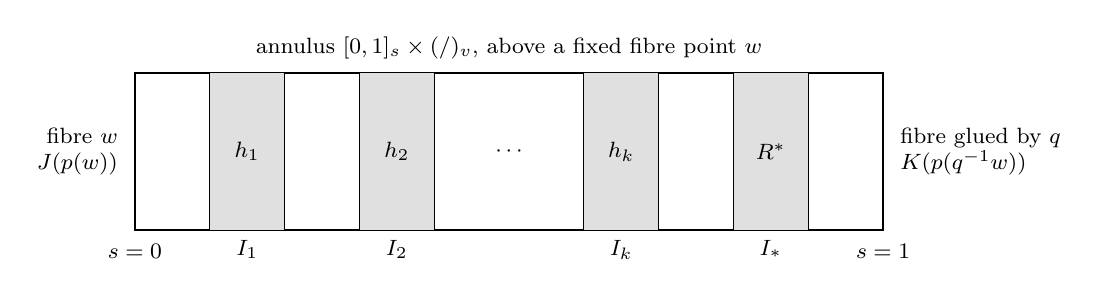
\begin{tikzpicture}[x=0.95cm,y=1cm,font=\footnotesize]
 \draw[thick] (0,0) rectangle (10,2);
 \foreach \l/\r/\t in {1/2/{h_1},3/4/{h_2},6/7/{h_k},8/9/{R^*}} {
  \fill[black!12] (\l,0) rectangle (\r,2);
  \draw (\l,0) -- (\l,2); \draw (\r,0) -- (\r,2);
  \node at ({(\l+\r)/2},1) {$\t$};
 }
 \node at (5,1) {$\cdots$};
 \node[below] at (1.5,0) {$I_1$}; \node[below] at (3.5,0) {$I_2$};
 \node[below] at (6.5,0) {$I_k$}; \node[below] at (8.5,0) {$I_*$};
 \node[below] at (0,-0.05) {$s=0$}; \node[below] at (10,-0.05) {$s=1$};
 \node[left,align=right] at (-0.1,1) {fibre $w$\\$J(p(w))$};
 \node[right,align=left] at (10.1,1) {fibre glued by $q$\\$K(p(q^{-1}w))$};
 \node[above] at (5,2.05) {annulus $[0,1]_s\times(\R/\Z)_v$, above a fixed fibre point $w$};
\end{tikzpicture}
\caption{The annulus above a fibre point $w$ in dimension four. The $\beta$-coefficient rises from $J(p(w))$ to
$K(p(q^{-1}w))$; across the layer $I_i$ it rises by the cap $h_i(p(w))$ of the $i$-th ball and across $I_*$ by the
positive remainder $R^*(w)$.}
\label{fig:mech-layers}
\end{figure}

\subsection{The comparison datum}\label{sec:mech-interfaces}

\begin{definition}[Comparison datum]\label{def:mech-datum}
A comparison datum for $([0,h],P)$ with gap $\gamma>0$ consists of a function $K$, smooth on a neighbourhood of
$[0,h]$, and a smooth Hamiltonian isotopy $(q_t)_{t\in[0,1]}$ of $\C$ with $q_0=\mathrm{id}$, generated by $Q_t$ with
$\iota_{X_{Q_t}}\omega_V=-dQ_t$, such that:
\begin{enumerate}[label=(\arabic*),ref=(\arabic*)]
\item\label{it:mech-datum-collar} $q_t(\bar D(h))=\bar D(h)$ for every $t$, and there is $\varsigma>0$ such that
 $Q_t=0$ on the collar $\{p>h-\varsigma\}$ for every $t$;
\item\label{it:mech-datum-cmp} $q=q_1$ satisfies the comparison inequality~\eqref{eq:mech-comparison}.
\end{enumerate}
\end{definition}

Section~\ref{sec:cmp} constructs the datum in closed form for equal balls with $k\ge10$ and $\frac34<\rho\sqrt k<1$
(Proposition~\ref{prop:cmp-linear}). Comparison data over polytopes, for general concave profiles, are constructed
in~\cite{SongHD}.
